\documentclass{resume} % Use the custom resume.cls style

\usepackage[left=0.75in,top=0.6in,right=0.75in,bottom=0.6in]{geometry} % Document margins
\usepackage{xcolor}
\usepackage{hyperref}
\hypersetup{
    colorlinks=true,
    linkcolor=blue,
    filecolor=magenta,      
    urlcolor=teal,
}
\usepackage{graphicx}
\newcommand{\tab}[1]{\hspace{.2667\textwidth}\rlap{#1}}
\newcommand{\itab}[1]{\hspace{0em}\rlap{#1}}
\name{Emilio Berti} % Your name
% \address{\centering 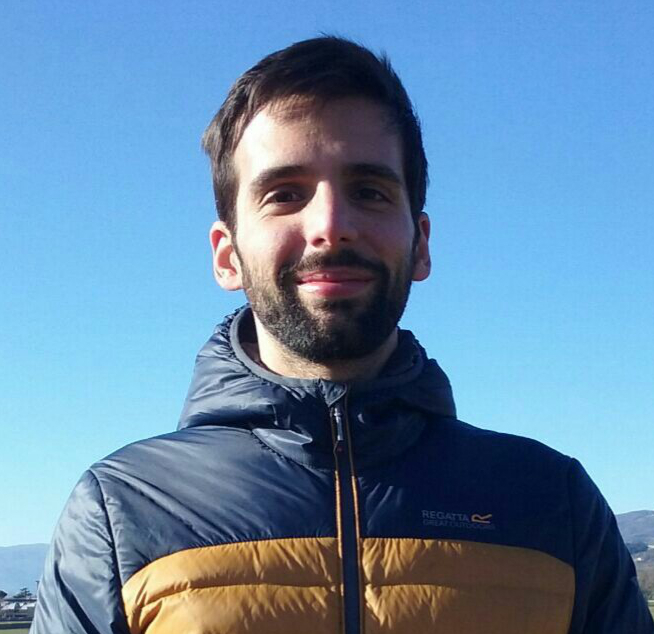
\includegraphics[width=0.30\textwidth]{Emilio.jpg}}
\address{
+49 1525 8953261\\ 
emilio.berti.academia@gmail.com\\ 
\href{https://scholar.google.com/citations?user=5KPh-oUAAAAJ&hl=en}{Google scholar} \\
\href{https://orcid.org/0000-0001-9286-011X}{ORCID} \\
\href{https://emilio-berti.github.io/}{website}
}

\begin{document}

\begin{rSection}{Summary}
I am a theoretical ecologist with a passion for math and computing. I have a strong quantitative background,
with expertise in mathematical and statistical modelling of complex systems using big databases at large
spatio-temporal scales. I have worked in many different fields of biology, from molecular muscle physiology
to macroecology and biogeography. I am very open minded to other cultures and societies: I am Italian,
my wife is Bulgarian, we met in Denmark, and we live in Germany. I am an avid reader of ancient history
and I love sumo.

\end{rSection}

\begin{rSection}{Professional experience}

{\bf PostDoctoral researcher} \hfill {\em October 2020 -- Present}\\
Theory in Biodiversity Science, German Centre for Integrative Biodiversity Research (\textsc{iDiv}), Leipzig, Germany.

{\bf Scientific consultant} \hfill {\em May 2020 -- July 2020}\\
Department of Bioscience, Aarhus University, Aarhus, Denmark.

{\bf Teaching assistant} \hfill {\em February 2017 -- April 2020}
\\Department of Biology, Aarhus University, Aarhus, Denmark.

\end{rSection}

\begin{rSection}{Education}
{\bf PhD} \hfill {\em February 2017 -- June 2020} \\
Section of Ecoinformatics and Biodiversity, Department of Biology, Aarhus University, Aarhus, Denmark.

{\bf Visiting PhD student} \hfill {\em Fall 2018} \\
Department of Ecology and Evolution, University of Chicago, Chicago, IL.

{\bf MSc in Biology} \hfill {\em 2013 -- 2016} \\
Department of Ecology and Evolution, University of Florence, Florence, Italy.

{\bf BSc in Biology} \hfill {\em 2009 -- 2012} \\
Department of Physiology, University of Florence, Florence, Italy.
\end{rSection}

\begin{rSection}{Grants}
\begin{tabular}{l l}
{\em 2024} & U. S. National Science Foundation (NSF). Understanding impacts of climatic variability on\\
           & distributions of species. 800,000\$ awarded to Prof. Daniel Reuman (PI), Emilio Berti (co-PI),\\
           & Townsend Peterson (co-PI), and Jorge L. Soberon (co-PI).
\end{tabular}
\end{rSection}

\begin{rSection}{Relevant skills}
I have developed an outstanding mathematical and theoretical set of skills and successfully applied it to
investigate macroecological and biogeographical drivers of biodiversity.

\textbf{Programming languages} – R, python, bash, C/C++, Stan, javascript (mostly for Google Earth Engine), SQL (postgis flavor).\\
\textbf{Software} – Linux/GNU, Anaconda, RShiny, Google Earth Engine, High-performance computing (HPC, Slurm flavor), Tidyverse, Git, GitHub, Jupyter Notebooks, \LaTeX.\\
\textbf{Methods} – Mathematical modeling, Geographic information systems (GIS), Geoinformatics, Geomatics, Remote sensing, Biostatistics, Data science, Climate analyses, Species distribution modeling, Environmental niche modeling, Machine learning, Bayesian statistics, Ordination and classification, Network theory,
Community assembly, Optimization, Automation.\\
\textbf{Languages} – Italian (native), English (fluent), German (A1 $\rightarrow$ A2).
\end{rSection}

\begin{rSection}{R packages}
\begin{itemize}
    \setlength\itemsep{-0.5em}
    \item GHCNr: Download and process daily weather data from the Global Historical Climatology Network (GHCN) database. \url{https://cran.r-project.org/package=GHCNr}.
    \item enerscape: Compute Energy Landscapes (CRAN). Author, maintainer. \url{https://cran.r-project.org/package=enerscape}.
    \item ATNr: Run Allometric Trophic Networks Models (CRAN). Author. \url{https://cran.r-project.org/package=ATNr}.
\end{itemize}
\end{rSection}

\begin{rSection}{Selected publications}
A full list of my publications can be found at \url{https://scholar.google.com/citations?user=5KPh-oUAAAAJ&hl=en}.

\begin{enumerate}
    \setlength\itemsep{-0.5em}
    \item Li, J., Brose, U., Rosenbaum, B., Ryser, R., \& \textbf{Berti, E}. (2024). Decoding Information Flow and Sensory Pollution: A Systematic Framework for Understanding Species Interactions. \textit{Ecology Letters}. DOI: \href{https://doi.org/10.1111/ele.14522}{10.1111/ele.14522}
    \item Carter, N. H., Berti, E., Zuckerwise, A., \& Pradhan, N. M. B. (2024). Energetics‐based connectivity mapping reveals new conservation opportunities for the endangered tiger in Nepal. \textit{Animal Conservation}. DOI: \href{https://doi.org/10.1111/acv.12937}{10.1111/acv.12937}.
    \item Antunes, A. C., \textbf{Berti, E.}, \dots, \& Gauzens, B. (2024). Linking biodiversity, ecosystem function, and Nature’s contributions to people: a macroecological energy flux perspective. \textit{Trends in Ecology \& Evolution}. DOI: \href{https://doi.org/10.1016/j.tree.2024.01.004}{10.1016/j.tree.2024.01.004}.
    \item Gauzens, B., Brose, U., Delmas, E., \& \textbf{Berti, E}. (2023). ATNr: Allometric Trophic Network models in R. Methods in Ecology and Evolution.
    \item Wei, S., \textbf{Berti, E.}, Ma, D., Wu, Q., Peng, Y., Yuan, C., ... \& Yue, K. (2023). Global patterns and drivers of lead concentration in inland waters. \textit{Journal of Hazardous Materials}. DOI: \href{https://doi.org/10.1016/j.jhazmat.2023.132455}{10.1016/j.jhazmat.2023.132455}
    \item Bauer, B., \textbf{Berti, E.}, ... \& Brose, U. (2022). Biotic filtering by species’ interactions constrains food-web variability across spatial and abiotic gradients. \textit{Ecology letters}. DOI: \href{https://doi.org/10.1111/ele.13995}{10.1111/ele.13995}. (\texttt{Shared first authorship}).
    \item Grenié, M, \textbf{Berti, E.}, ... \& Marten, W. (2022). Harmonizing taxon names in biodiversity data: a review of tools, databases, and best practices. \textit{Methods in Ecology and Evolution}. DOI: \href{https://doi.org/10.1111/2041-210X.13802}{10.1111/2041-210X.13802}.
    \item \textbf{Berti, E.}, Davoli, M., ... \& Vollrath, F. (2021). The r package enerscape: A general energy landscape framework for terrestrial movement ecology. \textit{Methods in Ecology and Evolution}. DOI: \href{https://doi.org/10.1111/2041-210X.13734}{10.1111/2041-210X.13734}.
    \item \textbf{Berti, E.}, Monsarrat, S., Munk, M., Jarvie, S. \& Svenning, J.C. (2020). Body size is a good proxy for vertebrate charisma. \textit{Biological Conservation}. DOI: \href{https://doi.org/10.1016/j.biocon.2020.108790}{10.1016/j.biocon.2020.108790}.
    \item \textbf{Berti, E.} \& Svenning, J.C. (2020). Megafauna extinctions have reduced biotic connectivity worldwide. \textit{Global Ecology and Biogeography}. DOI: \href{https://doi.org/10.1111/geb.13182}{10.1111/geb.13182}.
\end{enumerate}
\end{rSection}

\begin{rSection}{Conference talks as presenter}
\begin{enumerate}
    \setlength\itemsep{-0.5em}
    \item \textbf{Berti, E.}, Rosenbaum, B., Brose, U., \& Vollrath, F. (2023). Energy landscapes direct the movement preferences of elephants. \textit{British Ecological Society annual meeting, Belfast, UK}/
    \item Bauer, B., \textbf{Berti, E.}, \dots, \& Brose, U. (2022). From regional to local scale: biotic interactions shape multilayer food-webs. \textit{SFE-GFO-EEF biannual meeting, Metz, France} (\underline{invited talk}).
    \item \textbf{Berti, E.}, \& Svenning, J.C. (2022). State-space models show that functional replacements of extinct megafauna have distinct habitat preference in a European rewilding area. \textit{SFE-GFO-EEF biannual meeting, Metz, France}.
    \item Grenié, M., \textbf{Berti, E.}, Carvajal-Quintero, J., Winter, M., \& Sagouis (2021). Matching Species Names Across Biodiversity Databases: Sources, tools, pitfalls and best practices for taxonomic harmonization. \textit{TDWG annual meeting, online}.
    \item \textbf{Berti, E.} \& Svenning, J.C. (2019). Megalinkers extinction and the decrease of ecosystem connectivity. \textit{ESA annual meeting, Louisville, KY}.
    \item \textbf{Berti, E.}, Jarvie, S. W., \& Svenning, J.C. (2018). Rewiring food webs via trophic rewilding. \textit{BES annual meeting, Belfast, UK}.
\end{enumerate}
\end{rSection}

\end{document}
